% Admitted by research/round28/advisor/ah1-gate.json after final skeptical review.
\section{HNM AH1: complete physical enrichment on a larger open graph\workstar}
AH1 reconstructs the open $3\times2\times1$-cell graph, its strict physical electric projection and every individually resolved channel in the specified enrichment. The graph has 24 vertices, 46 links and 29 faces, including seven internal faces. The initial projection has rank 30; the enriched physical space has rank 561, a positive exact Haar Gram and 2,124 nonzero retained magnetic entries. For the contracted preparation class, the exact full and retained heat evolutions, each centered at its own actual ground energy, have all-time true-output-relative error below $11/5000=0.0022$. This is an analytic certificate, not a numerical heat trajectory or a graph-size-uniform result.

\subsection{Every original link, boundary gauge action and full domain}
The vertex set is $\{0,1,2,3\}\times\{0,1,2\}\times\{0,1\}$. Links are oriented in positive coordinate directions; a face with ordered axes $a<b$ follows the word $+a,+b,-a,-b$. The complete list has twelve $xy$, nine $xz$ and eight $yz$ faces. Its cycle rank $46-24+1=23$ is a graph invariant, not the dimension of a linear Wilson-function basis. All boundary vertices carry the gauge action
$U_{(v,w)}\mapsto g_vU_{(v,w)}g_w^{-1}$; a closed face word transforms by conjugation at its base. No tree links or original electric derivatives are deleted.

\begin{figure}[htbp]
 \centering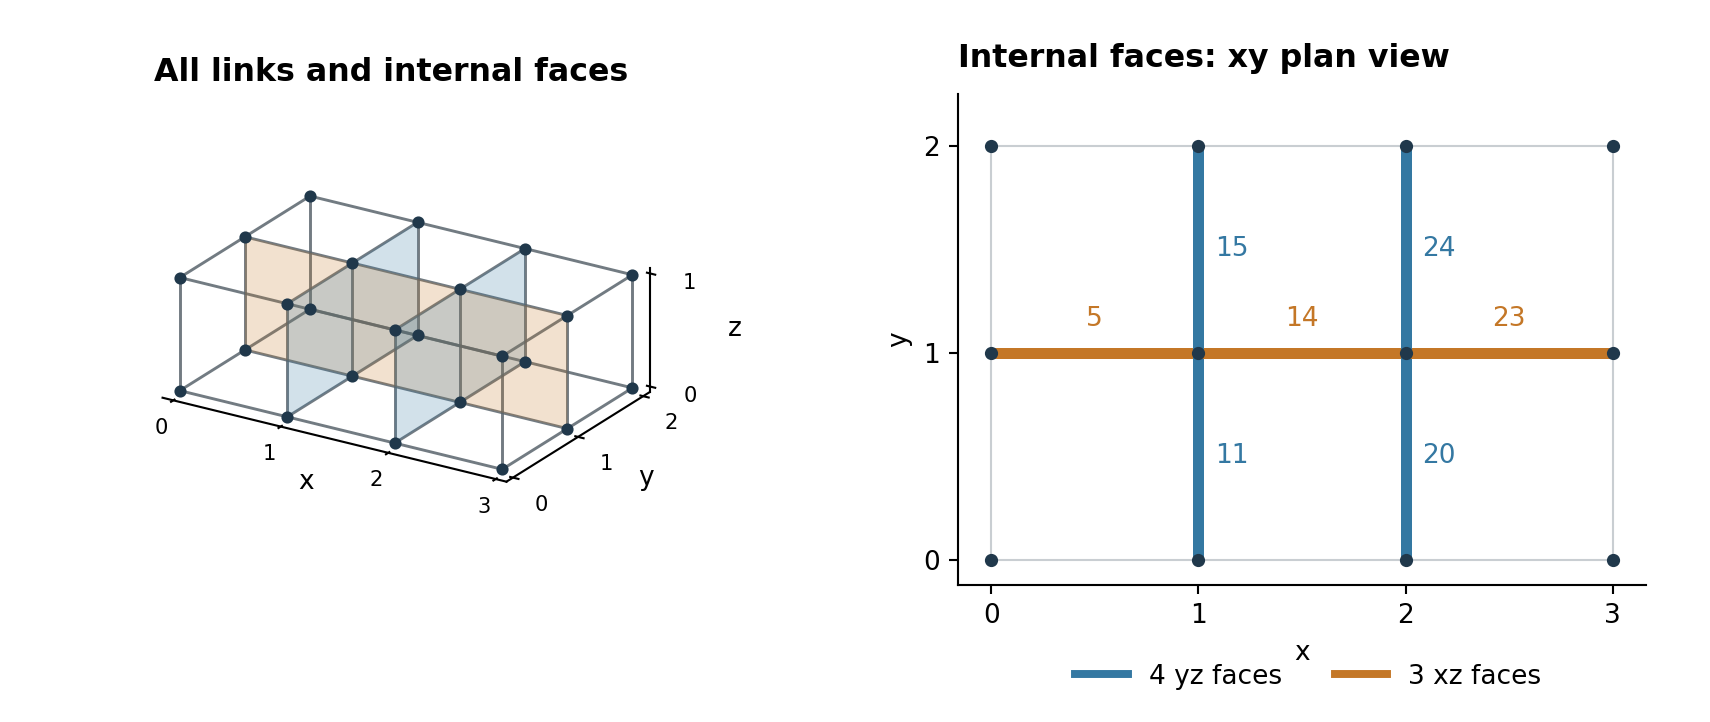
\includegraphics[width=.98\linewidth]{addenda/round28/figures/ah1-complete-graph.png}
 \caption{The actual AH1 coordinate graph and its seven internal faces. The left panel retains every one of the 46 links and 24 vertices. The right panel projects the seven vertical internal faces onto the $xy$ plane; numbers are frozen face IDs. Colors distinguish the two plane orientations. This is graph geometry, not a proposed physical apparatus or a heat simulation.}
 \label{r28:fig:ah1-graph}
\end{figure}

On normalized product Haar measure, the actual model is
\begin{align}
 \mathcal H_{\rm phys}&=L^2(\mathrm{SU}(2)^{46})^{\mathrm{SU}(2)^{24}},
 &K&=\sum_e C_e,\notag\\
 W_p&=\tfrac12\operatorname{Tr}U_{\partial p},
 &S&=\sum_{p=0}^{28}W_p,\qquad L=K+\lambda(29-S).
 \label{r28:eq:ah1-model}
\end{align}
Product Peter--Weyl labels give electric energies $\sum_ej_e(j_e+1)$ with finite multiplicities below every bound. Gauge averaging preserves each complete label block and commutes with the Casimirs. The restricted $K$ is self-adjoint with compact resolvent, operator domain the invariant product $H^2$ space, form domain invariant $H^1$, and smooth invariant Peter--Weyl core. Since $0\le29-S\le58$, bounded perturbation gives $D(L)=D(K)$ and the same form domain and compact resolvent. For the declared $0\le\lambda\le1/100$, $L\ge K$. These are full representation-space statements, not consequences of a finite matrix cutoff.

Physical energy is $H=\alpha L$, and heat time is $\sigma=\alpha t/\hbar$, with $a,E_*,\alpha/E_*,\hbar$ fixed and positive. This is a finite uniform-coupling graph model, distinct from the preceding homogeneous and canonical families. The theorem concerns Euclidean heat, not real-time evolution.

\subsection{The strict electric cutoff and actual Haar quotient}
Every nontrivial invariant spin support has no degree-one active vertex, and every active edge costs at least $3/4$. Below $9/2$ at most five edges are active. A nonempty such support contains a cycle; the graph is simple, bipartite and of girth four. Two components would require at least eight edges. A five-vertex, five-edge minimum-degree-two component would be an odd five-cycle, while a bipartite support on at most four vertices has at most four edges. Hence the only possible nonempty support is a four-cycle. Complete graph enumeration identifies these exactly with the 29 elementary faces.

At bivalent vertices the invariant tensor forces a common spin around the cycle. The strict inequality $4j(j+1)<9/2$ selects $j=1/2$, and its normalized function is $\phi_p=2W_p$. Therefore
\begin{equation}
 P_0=\mathbf1_{[0,9/2)}(K),\qquad
 \operatorname{ran}P_0=\operatorname{span}\{\Omega,\phi_0,\ldots,\phi_{28}\},
 \qquad\operatorname{rank}P_0=30.
 \label{r28:eq:ah1-strict}
\end{equation}
The electric vacuum is unique and its full physical gap is exactly three. Six-edge fundamental loops have energy exactly $9/2$ and are excluded from this initial interval. A total spin-degree cutoff is not identified with it.

For $p<q$ put $X_{pq}=W_pW_q$. There are 96 pairs sharing one edge and 310 sharing no edge; 64 of the latter meet only at vertices. On a common edge let $E_e$ be Haar integration, the spin-zero Casimir projection, and split $X_s=E_eX_{pq}$, $X_t=X_{pq}-X_s$. These are the two generated branches of $1/2\otimes1/2=0\oplus1$. Haar averaging commutes with the endpoint gauge actions. With the face orientations retained, the basic conditional identity is
\begin{equation}
 \int\chi(AU)\chi(U^{-1}B)\,dU=\tfrac12\chi(AB).
 \label{r28:eq:ah1-haar}
\end{equation}
The two exterior three-link paths use disjoint variables. Their conditional Haar norms give $\norm{X_s}^2=1/64$, $\norm{X_t}^2=3/64$ and zero cross term. Exact quaternion-polynomial integrations check this result; no Monte Carlo or joint independence of all face holonomies is assumed.

The specified \emph{individually resolved} enrichment consists of these actual functions:
\begin{center}\small
\begin{tabular}{@{}lrrr@{}}\toprule
Function & Count & Squared norm & Electric energy\\\midrule
$\Omega$&1&1&0\\
$\phi_p=2W_p$&29&1&3\\
$\chi_p=4W_p^2-1$&29&1&8\\
$d_{pq}=4W_pW_q$, edge-disjoint&310&1&6\\
$s_{pq}=8X_s$, shared edge&96&1&$9/2$\\
$t_{pq}=8X_t$, shared edge&96&3&$13/2$\\\bottomrule
\end{tabular}
\end{center}
Every one of the 406 pair parity masks is nonzero, distinct from the others and unequal to a single-face mask. Independent edge-center flips prove the corresponding orthogonalities; spin-one face characters are separately distinguished by their integer representation supports. The two shared branches are orthogonal electric eigenspaces. Thus the actual Gram is diagonal with 465 ones and 96 threes, has zero kernel, and gives quotient rank 561. This is proved from the graph and Haar functions, not assumed from an older example. Smooth electric eigenvectors make the resulting orthogonal $P_+$ reduce $K$ and its operator and form domains. The span does not fill complete ambient electric shells, and taking only the cyclic closure of summed columns need not separate its individual degenerate channels.

\subsection{The complete magnetic matrix and simultaneous outside loading}
Assign link-center signs $+1$ on $x$ links, $(-1)^x$ on $y$ links and $(-1)^{x+y}$ on $z$ links. Their product is $-1$ on every actual face. This Haar-preserving transformation commutes with $K$ and gauge averaging and sends $S$ to $-S$. Vacuum and the quadratic channels are even; the fundamental faces are odd. It proves all same-parity magnetic entries vanish. The pair-mask independence above is a separate argument.

The complete old columns are
\begin{align}
 S\Omega&=\tfrac12\sum_p\phi_p,\notag\\
 S\phi_p&=\tfrac12\Omega+\tfrac12\chi_p
 +\tfrac12\sum_{q:\,e(p)\cap e(q)=\varnothing}d_{pq}
 +\tfrac14\sum_{q:\,|e(p)\cap e(q)|=1}(s_{pq}+t_{pq}).
 \label{r28:eq:ah1-all-columns}
\end{align}
Together with the parity zeros and metric self-adjointness $g_iS_{ij}=g_jS_{ji}$, these determine every retained magnetic entry. In particular a triplet-to-face coefficient is $3/4$, while its face-to-triplet coefficient is $1/4$. Blind coordinate transposition would be wrong. The exact sparse export contains 2,124 directed nonzero entries and a defining zero rule for the other 312,597 entries. The full retained generator is its sum with the listed electric diagonal and $29\lambda I$.

For $A_+=P_+LP_+$ and $Q_+=I-P_+$, define the actual full outside map
\begin{equation}
 B=Q_+LP_+=-\lambda Q_+SP_+,
 \qquad BP_0=0,
 \qquad\norm B\le29\lambda.
 \label{r28:eq:ah1-outside}
\end{equation}
K reduction and \eqref{r28:eq:ah1-all-columns} justify the first two statements. Orthogonal projection in the actual physical Gram and $\norm S\le29$ give the last bound simultaneously for every complex retained input. Every new column and unretained intertwiner is charged. Equivalently, for each basis function $b_j$ its outside column is the full polynomial
$-\lambda[Sb_j-\sum_i b_i\langle b_i,Sb_j\rangle/g_i]$.
This specifies all columns without claiming an evaluated cubic outside Gram or exact outside norm.

The map is nonzero for $\lambda>0$: the normalized spin-$3/2$ same-face character $\xi_p$ has energy 15 and lies outside $P_+$, with
\begin{equation}
 \langle\xi_p,B\chi_p\rangle=-\lambda/2.
\end{equation}
Other faces have the wrong center mask for this coefficient. Thus $BP_0=0$ does not give autonomous retained dynamics; newly populated channels can load the exterior.

\subsection{The full original residual and both nested ground comparisons}
Put $m=29$ and
\begin{align}
 w=\frac{\sqrt{9+m\lambda^2}-3}{2},\qquad
 h&=\frac{\lambda}{2(3+w)},\qquad Z=1+mh^2,\notag\\
 f_0&=\frac{\Omega+h\sum_p\phi_p}{\sqrt Z},
 \quad\mu_0=m\lambda-w.
 \label{r28:eq:ah1-ritz}
\end{align}
These are the exact ground pair of the complete $P_0$ star matrix. The dark face eigenvalues are $3+m\lambda$. Positivity, compactness, the electric gap and min-max first establish unique full and compressed grounds with
\begin{equation}
 0\le\epsilon\le\mu_+\le\mu_0\le29\lambda<3,
 \qquad E_1(L),E_1(A_+),E_1(A_0)\ge3.
 \label{r28:eq:ah1-isolation}
\end{equation}
Thus isolation precedes residual inference. Write their rank-one projections as $G,G_+,G_0$.

For $F=S^2-m/4$, complete conditional Haar fourth moments and the pair masks yield
\begin{align}
 F&=\tfrac14\sum_p\chi_p+\tfrac12\sum_{\rm disjoint}d_{pq}
    +\tfrac14\sum_{\rm shared}(s_{pq}+t_{pq}),\notag\\
 \norm F^2&=\frac{m(2m-1)}{16}=\frac{1653}{16},\qquad
 (L-\mu_0)f_0=-\frac{2\lambda h}{\sqrt Z}F,\notag\\
 \rho_0^2&=\frac{1653\lambda^2h^2}{4Z}.
 \label{r28:eq:ah1-full-residual}
\end{align}
The original omitted-channel Gram has diagonal $m/4$, off-diagonal $1/4$, and bright/dark eigenvalues $57/4$ and $7$. It is independently recovered from the full resolved matrix. The residual above is the actual full-Hilbert residual; keeping only the spin-one face terms would miss most of it.

For the uniform coupling cap $\Lambda=1/100$, define
\begin{equation}
 g=3-29\Lambda=271/100,
 \qquad\bar r_0=41\Lambda^2/12,
 \qquad\bar p_0=\bar r_0/g.
\end{equation}
The inequalities $h\le\lambda/6$ and $\sqrt{1653}<41$ justify the first residual envelope. There are two distinct spectral arguments:
\begin{equation}
 \norm{G-G_0}\le\bar p_0,
 \qquad\norm{G_+-G_0}\le\bar p_0.
 \label{r28:eq:ah1-two-p0}
\end{equation}
The first uses the full spectral measure of $f_0$. For the second, $BP_0=0$ implies $Lf_0\in\operatorname{ran}P_+$, so the residual in the separately isolated $A_+$ spectrum is exactly the same full residual. An internal zero residual of the enriched ground would not replace either argument.

For the exact normalized enriched ground $f_+$, $BG_0=0$ then gives
\begin{equation}
 \rho_+=\norm{(L-\mu_+)f_+}=\norm{B(I-G_0)f_+}
 \le29\Lambda\bar p_0=:\bar r_+.
\end{equation}
Its full spectral measure and the nonnegative spectral polynomial $(L-\epsilon)(L-3)$ give
\begin{equation}
 \norm{G-G_+}\le\bar p_+:=\bar r_+/g,
 \qquad0\le\mu_+-\epsilon\le\bar d_+:=\bar r_+^2/g.
 \label{r28:eq:ah1-plus-residual}
\end{equation}
Smoothness supplies the second moment needed for the energy estimate. All barred quantities are upper envelopes, not evaluated actual enriched ground data. In exact fractions,
\begin{equation}
 \bar p_0=\frac{41}{325200},\qquad
 \bar r_+=\frac{1189}{32520000},\qquad
 \bar p_+=\frac{1189}{88129200},\qquad
 \bar d_+=\frac{1413721}{2865961584000000}.
\end{equation}

\subsection{True output denominator and independently centered heat}
Let $x$ be any normalized complex vector in $\operatorname{ran}P_0$ with $\norm{x-\Omega}\le\eta=1/100$. Following the forward constants, put
\begin{align}
 z_0=1-29\Lambda^2/72,\qquad q_0=(11/12)\Lambda,\qquad
 b&=q_0+\bar p_0+\eta,\notag\\
 D&=z_0-\eta-\bar p_0=\frac{193136341}{195120000}>0.
 \label{r28:eq:ah1-true-floor}
\end{align}
The Ritz overlap and both comparisons in \eqref{r28:eq:ah1-two-p0} give
$\norm{(I-G)x},\norm{(I-G_+)x}\le b$. For the actual full heat,
\begin{equation}
 E(\sigma)=e^{-\sigma(L-\epsilon)},\qquad
 E_+(\sigma)=e^{-\sigma(A_+-\mu_+)}P_+,
 \qquad\norm{E(\sigma)x}\ge\norm{Gx}\ge D.
 \label{r28:eq:ah1-heats}
\end{equation}
The denominator is the true full output, not a Ritz norm or a regularizer. The bounds apply to complex preparations and both centered excited gaps are at least $g$.

Strong differentiation on smooth finite retained vectors and vectorwise integration give the exact identity
\begin{equation}
 (E-E_+)(\sigma)x=-\int_0^\sigma E(\sigma-s)
 [B+(\mu_+-\epsilon)P_+]E_+(s)x\,ds.
 \label{r28:eq:ah1-duhamel}
\end{equation}
The full $E$ inside the integral retains outside evolution and return. The plus centering defect survives $BP_0=0$. No unbounded operator-norm derivative is assumed. Independent ground/excited decompositions give an increasing early bound and decreasing late bound,
\begin{align}
 V(\sigma)&=(\bar r_++\bar d_+)\sigma
       +\frac{29\Lambda b}{g}(1-e^{-g\sigma}),\notag\\
 J(\sigma)&=\bar p_++(2b+\bar p_+)e^{-g\sigma}.
 \label{r28:eq:ah1-join-bounds}
\end{align}
The extra decaying $\bar p_+$ term is harmless slack. At the predeclared join $\sigma=2$, use $1-e^{-2g}\le1$ and a positive rational Taylor sum proving $e^{2g}>225$. Monotonicity covers $[0,2]$ and $[2,\infty)$ without a time grid. The forward certificate is
\begin{equation}
 \sup_{\sigma\ge0}
 \frac{\norm{(E-E_+)(\sigma)x}}{\norm{E(\sigma)x}}
 \le\frac{3063228992521}{1418412601938100}
 <\frac{11}{5000}.
 \label{r28:eq:ah1-main-bound}
\end{equation}
The skeptic independently reaches the same rational headline. The reverse proof uses the tighter valid $q_0=(9/10)\Lambda$ and obtains
$3037671524521/1418412601938100<43/20000=0.00215$.
These are conservative exact-semigroup bounds, not measured approximation errors; the larger graph's common certificate is weaker than the earlier graph's sharper AC2 certificate.

At zero time the two exact evolutions agree on this initial class. At zero coupling they agree on retained inputs at every time because $P_+$ reduces $K$. Those exact statements supersede positive cap envelopes. Zero-extension has full-input operator norm error one at zero time, so arbitrary full-Hilbert initial accuracy is not claimed. Replacing either actual ground center by $29\lambda$ or by an independently rounded energy can produce long-time exponential error and is outside the theorem.

Exact controls test the actual gauge words, every internal face, the strict endpoint, both shared branches, the triplet metric, duplicate-coordinate null relations, individual versus summed channels, new-input spin-$3/2$ leakage, negative-coupling misuse, complex preparations and center-shift sign. The reverse record preserves an initially nondiscriminating orientation fixture and its discriminating replacements; that control refinement adds no investigation. Exact generator actions are executed, but no numerical heat evaluator or numerical trajectory is supplied. Such an implementation would require an added error budget divided by the same true denominator. The outside cubic Gram, complete ambient-shell enrichment, real-time relative control, volume-uniform limit, canonical/homogeneous matching and continuum Yang--Mills mass gap remain open; scientific priority is unverified.
